\section{Диаграммы IDEF0}
    \subsection{Контекстная диаграмма верхнего уровня}
    \begin{figure}[H]
        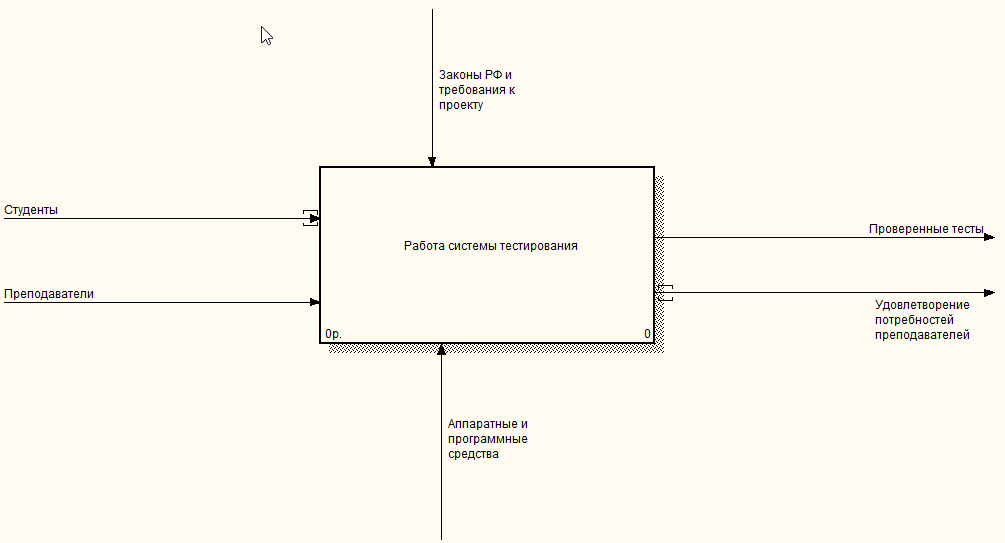
\includegraphics[width=\textwidth, center]{../img/idef0/idef0_context.png}
        \caption{Контекстная диаграмма верхнего уровня}
    \end{figure}

    Данная диаграмма является общим представлением работы автоматизированной
    системы для тестирования.

    На вход системы поступают преподаватели (администрароторы) и студенты
    (пользователи).

    Выходными блоками являются проверенные тестовые задания и удовлетворенные
    потребности преподавателей.

    Управление для данной системы осуществляют законы Российской Федерации,
    устанавливающие порядок обработки персональных данных, а также ряд других
    ограничений, и требования, предъявляемые к функциональности системы.

    Механизмами, выполняющими преобразования входных данных в выходные являются
    аппаратные и программные средства: компьютеры, операционная система,
    языки программирования, различные библиотеки и виртуальные среды для
    выполнения кода программы.

    \subsection{Работа системы тестирования}
    \begin{figure}[H]
        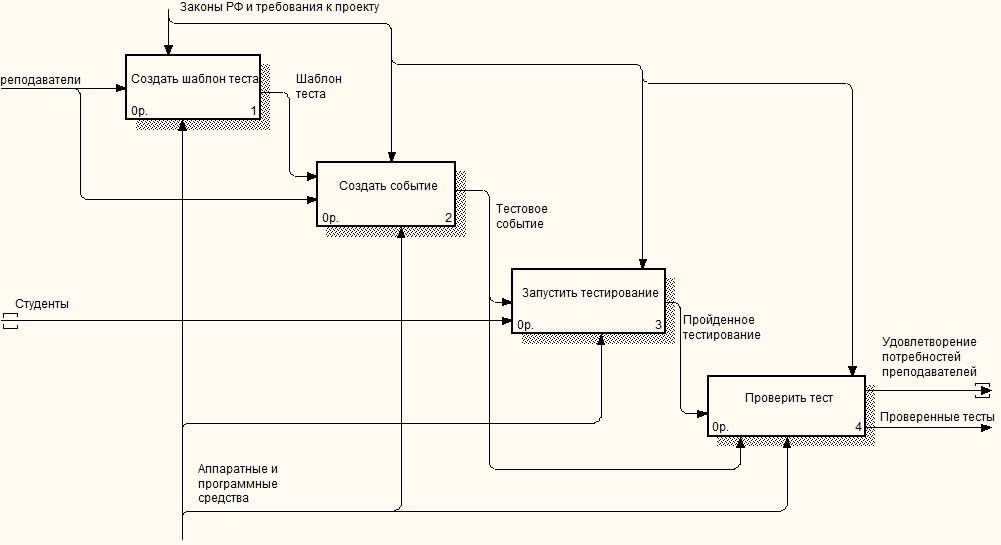
\includegraphics[width=\textwidth, center]{../img/idef0/context_decompose.png}
        \caption{Работа системы тестирования}
    \end{figure}

    Данная диаграмма раскрывает функциональный блок контекстной
    диаграммы верхнего уровня "Работа системы тестирования".

    На диаграмме представлены следующие функциональные блоки:
    \begin{enumerate}
        \item Создать шаблон теста - на вход получает преподавателей, а на выходе имеет 
        шаблон тестовый шаблон
        \item Создать событие - принимает на вход преподавателей и созданный тестовый
        шаблон и возвращает тестовое событие
        \item Запустить тестирование - получает тестовое событие и студентов, а
        выдает пройденное тестирование
        \item Проверить тест - Преобразует пройденное тестирование в проверенное
        тестирование и удовлетворение потребностей преподавателей.
    \end{enumerate}

    Далее будут более подробно рассмотрены представленные функциональные блоки.

    \subsection{Создать шаблон теста}
    \begin{figure}[H]
        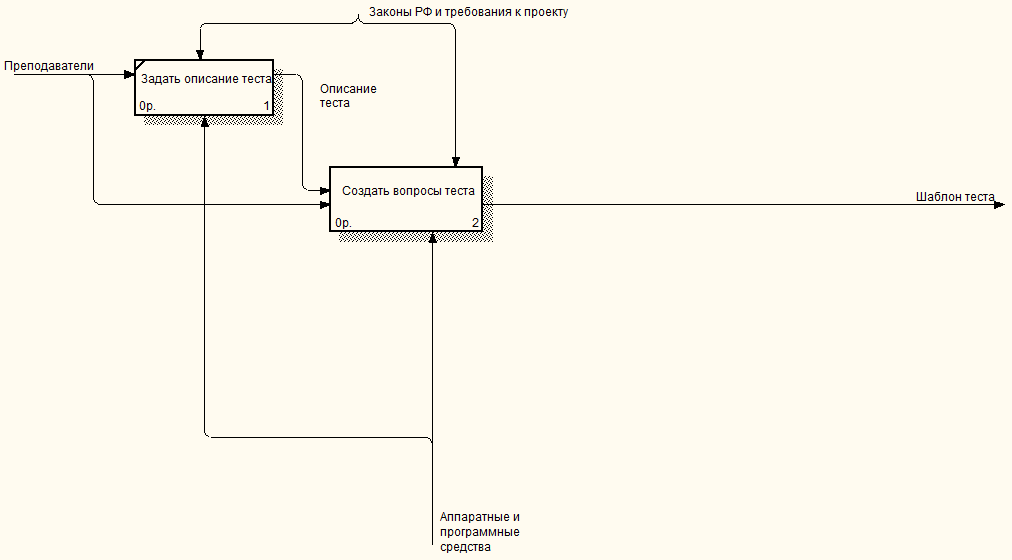
\includegraphics[width=\textwidth, center]{../img/idef0/CreateTestTemplate.png}
        \caption{Создать шаблон теста}
    \end{figure}

    На диаграмме представлены следующие функциональные блоки:
    \begin{enumerate}
        \item Задать описание теста - на вход принимает преподавателей, а на выходе
        имеет описание теста
        \item Создать вопросы теста - на вход принимает преподавателей и описание теста,
        а на выходе имеет шаблон теста
    \end{enumerate}


    \subsection{Создать вопросы теста}
    \begin{figure}[H]
        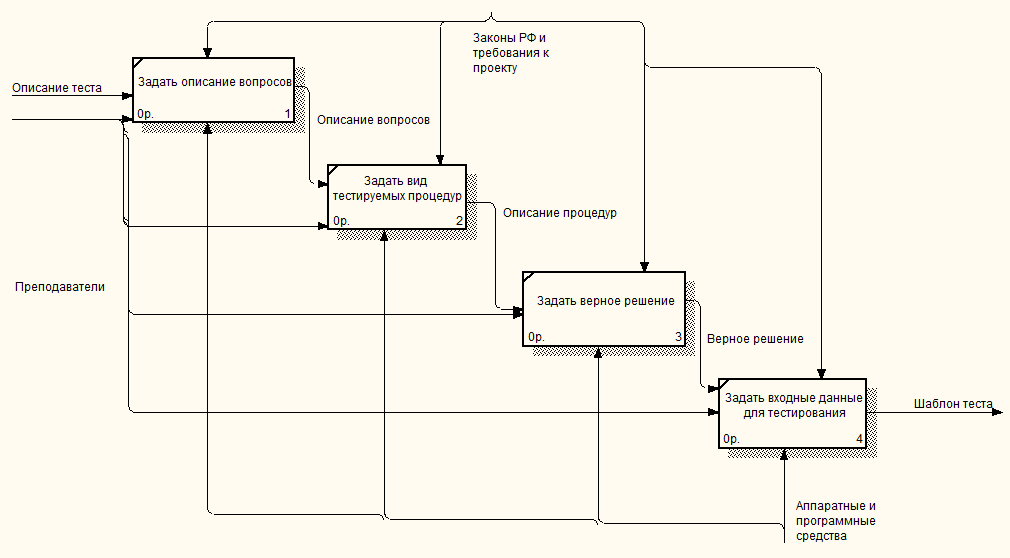
\includegraphics[width=\textwidth, center]{../img/idef0/CreateTemplateQuestions.png}
        \caption{Создать шаблон теста}
    \end{figure}
    \begin{enumerate}
        \item Задать описание вопросов - на вход принимает описание тестов и преподавателей,
        а на выходе имеет описание вопросов
        \item Задать вид тестируемых процедур - на вход принимает преподавателей и
        описание вопросов, а на выходе имеет описание процедур
        \item Задать верное решение - на вход принимает преподавателей и описание процедур,
        а на выходе имеет верное решение
        \item Задать входные данные для тестирование - на вход принимает верное решение
        и преподавателей, а на выходе имеет шаблон теста
    \end{enumerate}

    \subsection{Создать событие}
    \begin{figure}[H]
        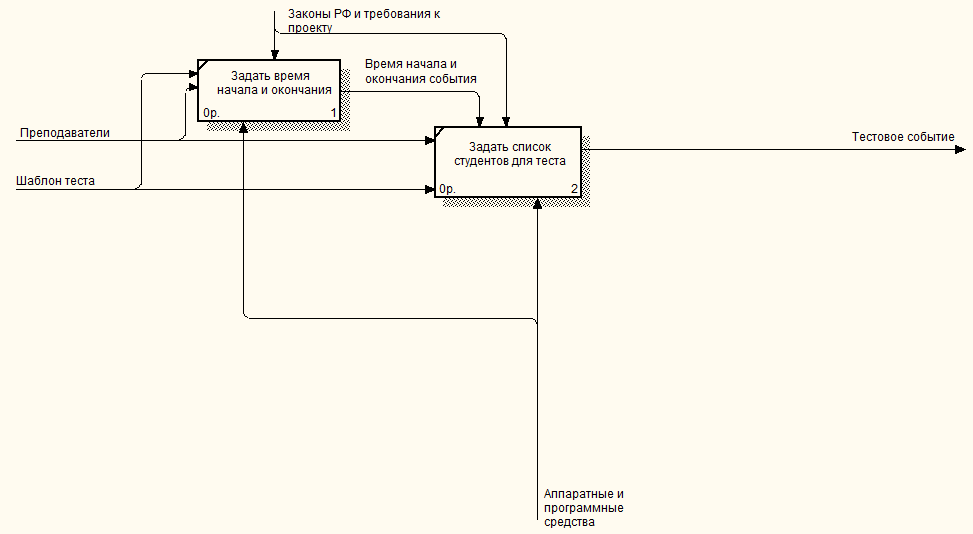
\includegraphics[width=\textwidth, center]{../img/idef0/CreateInstance.png}
        \caption{Создать событие}
    \end{figure}
    
    \begin{enumerate}
        \item Задать время начала и окончания - на вход принимает преподавателей и
        шаблон теста, а на выходе имеет время начала и окончания события
        \item Задать список студентов и для теста - на вход принимает преподавателей
        и шаблон теста, а на выходе имеет тестовое событие
    \end{enumerate}

    \subsection{Запустить тестирование}
    \begin{figure}[H]
        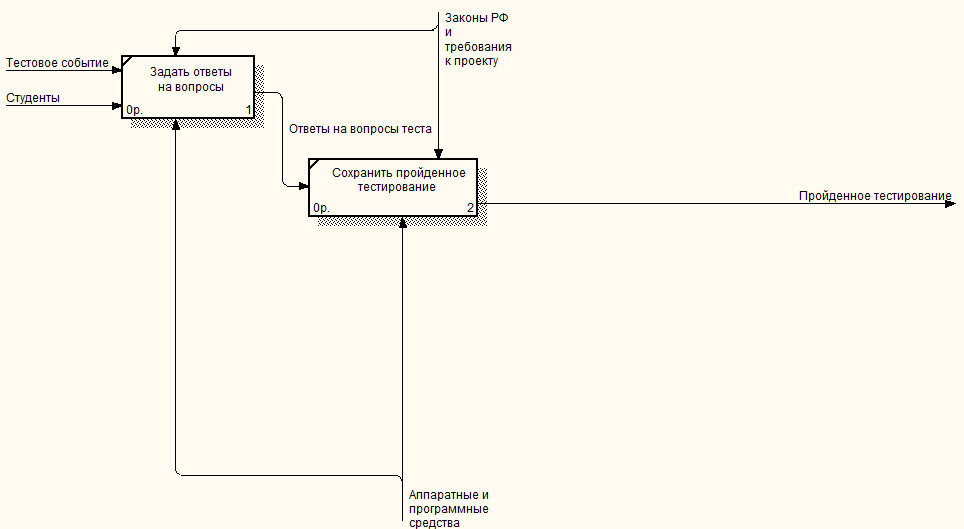
\includegraphics[width=\textwidth, center]{../img/idef0/RunTestDecompose.png}
        \caption{Запустить тестирование}
    \end{figure}

    \begin{enumerate}
        \item Задать ответы на вопросы - на вход принимает тестовое событие и
        студентов, а на выходе имеет ответы на вопросы теста
        \item Сохранить пройденное тестирование  - на вход принимает ответы
        на вопросы теста, а на выходе имеет пройденное тестирование
    \end{enumerate}

    \subsection{Проверить тест}
    \begin{figure}[H]
        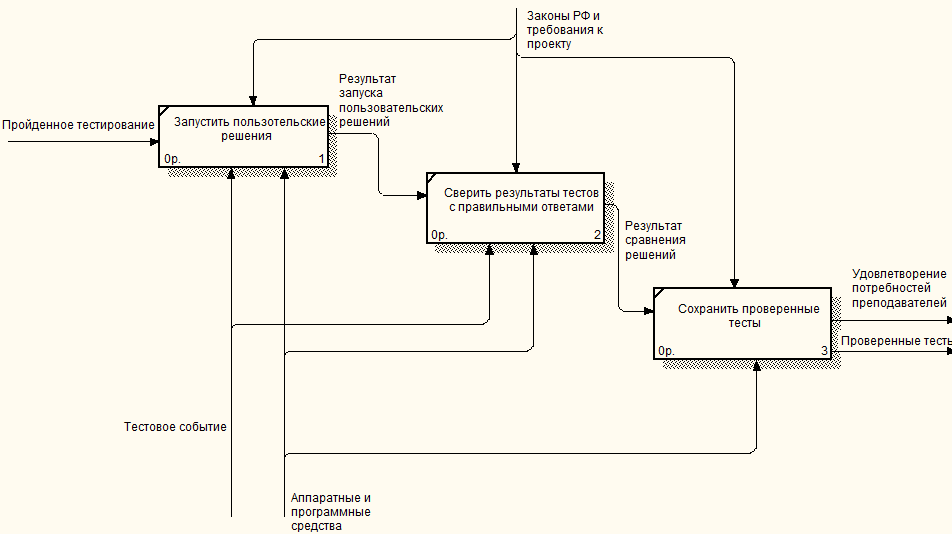
\includegraphics[width=\textwidth, center]{../img/idef0/ValidateTestDecompose.png}
        \caption{Проверить тест}
    \end{figure}

    \begin{enumerate}
        \item Запустить пользовательские решения - на вход принимает пройденное тестирование,
        а на выходе имеет результат запуска пользовательских решений
        \item Сверить результаты тестов с правильными ответами - на вход принимает 
        результат запуска пользовательских решений, а на выходе имеет результат сравнения 
        решений
        \item Сохранить проверенные тесты - на вход принимает результат сравнения
        решений, а на выходе имеет проверенные тесты и удовлетворение потребностей
        преподавателей
    \end{enumerate}

    \subsection{Запустить пользовательские решения}
    \begin{figure}[H]
        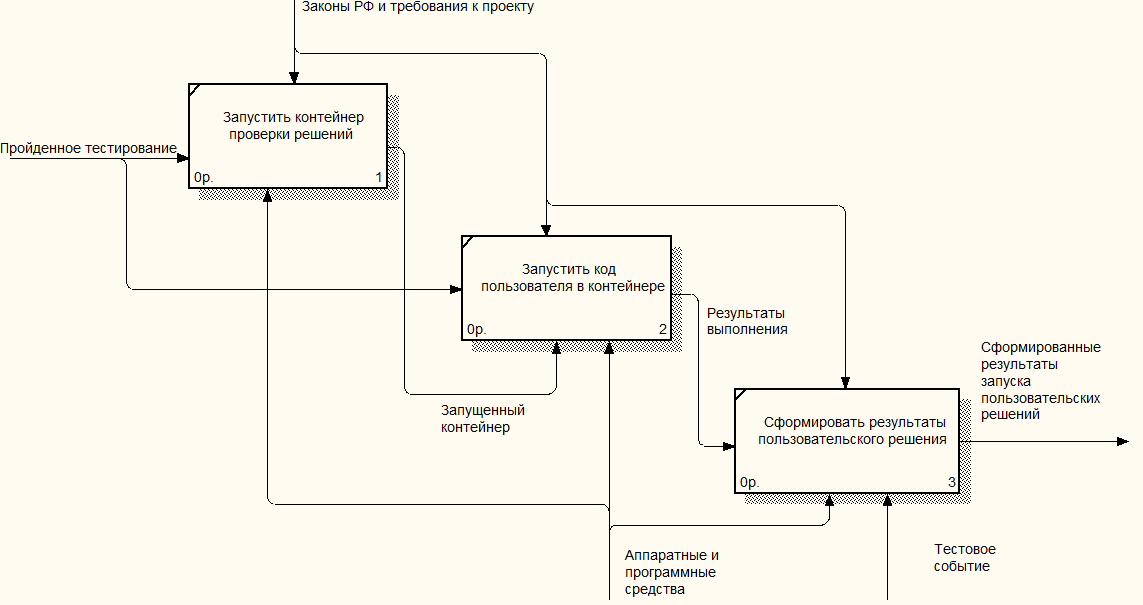
\includegraphics[width=\textwidth, center]{../img/idef0/RunUserSolutionsDecompose.png}
        \caption{Проверить тест}
    \end{figure}
    \begin{enumerate}
        \item Запустить контейнер проверки решений - на вход принимает пройденное тестирование, а на выходе имеет запущенный контейнер.
        \item Запустить код пользователя в контейнере - на вход принимает пройденное тестирование, механизмом является запущенный контейнер, а на выходе имеет результаты выполнения пользовательского кода.
        \item Сформировать результаты пользовательского решения - на вход поступают результаты выполнения пользовательского кода, а на выходе имеет сформированные результаты запуска пользовательских решений.
    \end{enumerate}